\documentclass{article}

\usepackage[utf8]{inputenc}
\usepackage{amsthm}
\usepackage{amssymb}
\usepackage{mathtools}
\usepackage{graphicx}
\usepackage{mdframed}
\usepackage{float}
\usepackage[top=1in, bottom=1.25in, left=1.25in, right=1.25in]{geometry}

\DeclarePairedDelimiter{\abs}{\lvert}{\rvert}
\DeclarePairedDelimiter{\norm}{\lvert \lvert}{\rvert \rvert}

\newtheoremstyle{break}% name
  {}%         Space above, empty = `usual value'
  {}%         Space below
  {\itshape}% Body font
  {}%         Indent amount (empty = no indent, \parindent = para indent)
  {\bfseries}% Thm head font
  {.}%        Punctuation after thm head
  {\newline}% Space after thm head: \newline = linebreak
  {}%         Thm head spec

\newtheorem{Def}{Definition}[section]

\theoremstyle{break}

\newtheorem{innerEx}{Exempel}[section]
\newtheorem{sats}{Sats}[section]
\newtheorem{Rem}{Anmärkning}[section]

\newenvironment{Ex}
{\begin{mdframed} \begin{innerEx} \vspace{3pt}}
{\vspace{3pt} \end{innerEx} \end{mdframed}}  

\newenvironment{bevis}
{\begin{mdframed} \begin{proof} \vspace{3pt}}
{\vspace{3pt} \end{proof} \end{mdframed}}

\title{
	Linjär Algebra\\
	Föreläsning 2
	\author{Erik Sjöström}
}

\begin{document}

\maketitle

\section{Skalärprodukten} % (fold)
\label{sec:skal_rprodukten}

Låt $\vec{u}$, $\vec{v}$ vara två vektorer. \underline{Skalärprodukten} definieras då som:
\begin{equation}
    \vec{u} \cdot \vec{v} = \norm{\vec{u}} \cdot \norm{\vec{v}} \cdot \cos{\theta}
\end{equation}
där $\theta$ är vinkeln mellan vektorerna.
\begin{Ex}
    \[
        \vec{u} \cdot \vec{u} = \norm{\vec{u}} \cdot \norm{\vec{u}} \cdot \cos{\theta} = \norm{\vec{u}}^2
    \]
\end{Ex}
\begin{Ex}
    Anta att vi har $\vec{u}$, $\vec{v}$ $\neq$ \O, och vinkeln mellan dem är $\theta$. Om:
    \[
        \vec{u} \cdot \vec{v} = 0 \Leftrightarrow \norm{\vec{u}} \cdot \norm{\vec{v}} \cdot \cos{\theta} = 0
    \]
    Dvs: $\cos{\theta} = 0$, vilket betyder att $\theta = \frac{\pi}{2} = 90^o$. \\
    Om $\vec{u}$ $\cdot$ $\vec{v}$ = 0, innebär det att $\vec{u}$ och $\vec{v}$ är ortogonala.
\end{Ex}
\noindent
Det gäller att:
\begin{itemize}
  \item $\vec{u} \cdot \vec{v} > 0 \Leftrightarrow$ Vinkeln spetsig
  \item $\vec{u} \cdot \vec{v} < 0 \Leftrightarrow$ Vinkeln trubbig
\end{itemize}

Säg att:

\[
    \vec{u} = \begin{bmatrix} u_1 \\ u_2 \end{bmatrix}, \vec{v} = \begin{bmatrix} v_1 \\ v_2 \end{bmatrix}, \vec{w} = \vec{u} - \vec{v} = \begin{bmatrix} u_1 - v_1 \\ u_2 - v_2 \end{bmatrix}
\]
\noindent
Då säger cosinus-satsen att:
\begin{alignat*}{3}
    \norm{\vec{w}}^2 &= \norm{\vec{u}}^2 + \norm{\vec{v}}^2 - 2 \cdot \norm{\vec{u}} \cdot \norm{\vec{v}} \cdot \cos{\theta} &&\Leftrightarrow\\
    \norm{\vec{u}} \cdot \norm{\vec{v}} \cdot \cos{\theta} &= \frac{1}{2} (\norm{\vec{u}}^2 + \norm{\vec{v}}^2 - \norm{\vec{w}}^2) &&\Leftrightarrow \\ 
    \vec{u} \cdot \vec{v} &= \frac{1}{2} ((u_1^2 + u_2^2) + (v_1^2 + v_2^2) - ((u_1-v_1)^2 + (u_2-v_2)^2)) \\
    &= \frac{1}{2} (u_1^2+u_2^2+v_1^2+v_2^2 - (u_1^2+v_1^2 - 2u_1v_1+u_2^2+v_2^2-2u_2v_2)) \\
    &= \frac{1}{2} (2u_1v_1 + 2u_2v_2)\\
    &= u_1v_1 + u_2v_2
\end{alignat*}
Dvs, om $\vec{u}$ = $\begin{bmatrix} u_1 \\ u_2 \end{bmatrix}$ och $\vec{v}$ = $\begin{bmatrix} v_1 \\ v_2 \end{bmatrix}$ är två vektorer i $\mathbb{R}^2$ så är:
\begin{equation}
    \vec{u} \cdot \vec{v} = u_1v_1 + u_2v_2
\end{equation}
Om $\vec{u}$ = $\begin{bmatrix} u_1 \\ u_2  \\ u_3 \end{bmatrix}$, $\vec{v}$ = $\begin{bmatrix} v_1 \\v_2\\v_3 \end{bmatrix}$ är vektorer i $\mathbb{R}^3$ så är:
\begin{equation}
  \vec{u} \cdot \vec{v} = u_1v_1 + u_2v_2 + u_3v_3      
\end{equation}
Detta härleds på samma sätt som för i $\mathbb{R}^2$.

% section skal_rprodukten (end)

\section{Projektion} % (fold)
\label{sec:projektion}

\begin{Def}
    Den ortogonala projektionen av vektor $\vec{v}$ på linjen L (med riktningsvektor $\vec{u}$) är den vektor som är parallell med $\vec{u}$ och så att ($\vec{v}$ - $\vec{v}_L$) är ortogonal mot L.
\end{Def}
\begin{center}
  \centering
  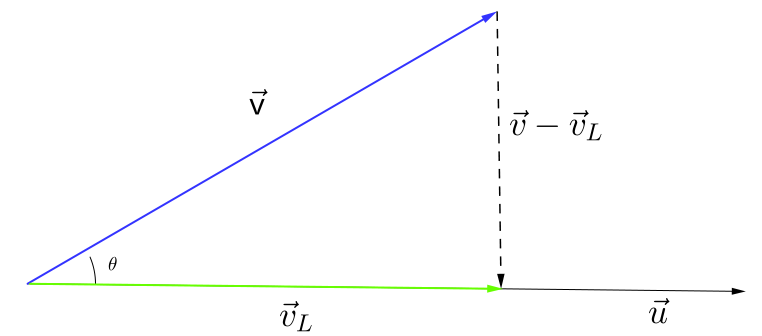
\includegraphics[scale=0.4]{projection.png}
\end{center}
\begin{Rem}
    $\norm{\vec{v}_L} = \norm{\vec{v}} \cdot \cos{\theta}$
\end{Rem}
\noindent
Det gäller att: $\vec{u} \cdot \vec{v}_L = \vec{u} \cdot \vec{v}$, när $\theta$ spetsig.\\
Ty:
\begin{align*}
    \vec{u} \cdot \vec{v}_L &= \norm{\vec{u}} \cdot \norm{\vec{v}_L} \cdot \cos{0}\\
    &= \norm{\vec{u}} \cdot \norm{\vec{v}_L} \\
    &= \norm{\vec{u}} \cdot \norm{\vec{v}} \cdot \cos{\theta} \\
    &= \vec{u} \cdot \vec{v}
\end{align*}
Analogt gäller det att: $\vec{u} \cdot \vec{v}_L = -(\vec{u} \cdot \vec{v})$, när $\theta$ trubbig.\\
Ty:
\begin{align*}
    \vec{u} \cdot \vec{v}_L &= \norm{\vec{u}} \cdot \norm{\vec{v}_L} \cdot \cos{\pi}\\
    &= \norm{\vec{u}} \cdot \norm{\vec{v}_L} \cdot (-1) \\
    &= \norm{\vec{u}} \cdot \norm{\vec{v}} \cdot \cos{\theta} \cdot (-1)\\
    &= -(\vec{u} \cdot \vec{v})
\end{align*}

\begin{sats}
    \begin{equation}
      \vec{v}_L = \frac{\vec{u} \cdot \vec{v}}{\vec{u} \cdot \vec{u}} \cdot \vec{u}
    \end{equation}
\end{sats}
\begin{bevis}
    Vi vet att:
    \[
    0 = \vec{u} \cdot \vec{v} - \vec{u} \cdot \vec{v}_L
    \]\\
    Vi får då att:
    \begin{align*}
    0 &= \vec{u} \cdot \vec{v} - \vec{u} \cdot \vec{v}_L \\
    &= \vec{u} \cdot \vec{v} -  \vec{u} \cdot (t \cdot \vec{u}) \\
    &= \vec{u} \cdot \vec{v} - t \cdot (\vec{u} \cdot \vec{u})
    \end{align*}
    Dvs: 
    \[
        \vec{u} \cdot \vec{v} = t \cdot (\vec{u} \cdot \vec{u})
    \]
    Lös ut $t$:
    \[
        t = \frac{\vec{u} \cdot \vec{v}}{\vec{u} \cdot \vec{u}}
    \]
    Eftersom $\vec{v}_L = t \cdot \vec{u}$ får vi att:
    \[
        \vec{v}_L = \frac{\vec{u} \cdot \vec{v}}{\vec{u} \cdot \vec{u}} \cdot \vec{u}
    \]

\end{bevis}
\newpage
\begin{sats}
  \begin{equation}
    \norm{\vec{v}_L} = \frac{\abs{\vec{u}\cdot \vec{v}}}{\norm{\vec{u}}}
  \end{equation}
\end{sats}
\begin{bevis}
    Vi vet att:
    \[
        \vec{v}_L = t \cdot \vec{u}
    \]
    för $t \in \mathbb{R}$, ty $\vec{v}_L$ är parallell med $\vec{u}$.\\
    Vi får då att:
    \begin{align*}
    \norm{\vec{v}_L} &= \norm{\vec{t \cdot \vec{u}}} \\
    &= \abs{t} \cdot \norm{\vec{u}} \\
    &= \abs{\frac{\vec{u} \cdot \vec{v}}{\vec{u} \cdot \vec{u}}} \cdot \norm{\vec{u}} \\
    &= \frac{\abs{\vec{u} \cdot \vec{v}}}{\norm{\vec{u}}^2} \cdot \norm{\vec{u}} \\
    &= \frac{\abs{\vec{u} \cdot \vec{v}}}{\norm{\vec{u}}}
    \end{align*}
    
\end{bevis}

% section projektion (end)

\section{Kryssprodukt} % (fold)
\label{sec:kryssprodukt}
\begin{Def}
    Givet 2 vektorer:
    \[
        \vec{u} = \begin{bmatrix} u_1 \\ u_2 \\ u_3 \end{bmatrix}, \vec{v} = \begin{bmatrix} v_1 \\ v_2 \\ v_3 \end{bmatrix}, \mbox{ i } \mathbb{R}^3
    \]
    Kryssprodukten definieras då som:
    \begin{equation}
        \vec{u} \times \vec{v} = \begin{bmatrix} u_2 \cdot v_3 - u_3 \cdot v_2 \\ u_3 \cdot v_1 - u_1 \cdot v_3 \\ u_1 \cdot v_2 - u_2 \cdot v_1\end{bmatrix}
    \end{equation}
    
\end{Def}
\begin{center}
  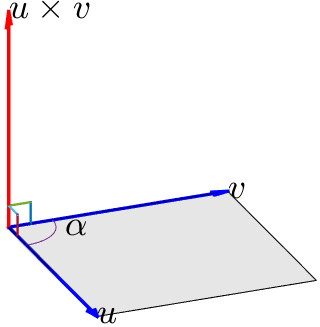
\includegraphics[scale=0.7]{kryssprodukt_08.png}
\end{center}
\samepage
\noindent

Egenskaper för kryssprodukten:
\begin{itemize}
  \item $\vec{u} \times \vec{u} =$\O
  \item $\vec{u} \times \vec{v} = -(\vec{v} \times \vec{u})$
  \item $(c \cdot \vec{u}) \times \vec{v} = c \cdot (\vec{u} \times \vec{v})$
  \item $\vec{u} \times (\vec{v} + \vec{w}) = \vec{u} \times \vec{v} + \vec{u} \times \vec{w}$
\end{itemize}
\begin{Ex}
    Om:
    \[
        \vec{u} = \begin{bmatrix} 1\\2\\3 \end{bmatrix}, \vec{v} = \begin{bmatrix} 1\\0\\2 \end{bmatrix}
    \]
    Så är:
    \[
        \vec{u} \times \vec{v} = \begin{bmatrix} 2 \cdot 2 - 3 \cdot 0\\3 \cdot 1 - 1 \cdot 2 \\ 1 \cdot0 - 2 \cdot 1 \end{bmatrix}
    \]
\end{Ex}
\begin{Ex}
    Finn en vektor som är ortogonal mot:
    \[
        \vec{u} = \begin{bmatrix} 1\\-1\\0 \end{bmatrix}, \mbox{ och } \vec{v} = \begin{bmatrix}0\\1\\-2  \end{bmatrix}
    \]
    Lösning:
    \[
        \vec{u} \times \vec{v} = \begin{bmatrix} (-1)(-2) - 0 \cdot 1\\0 \cdot 0 - 1 \cdot (-2)\\1 \cdot 1 - (-1) \cdot 0 \end{bmatrix} = \begin{bmatrix} 2\\2\\1 \end{bmatrix}
    \]
    Vi kan se att $\vec{u} \times \vec{v}$ är vår lösning ty:
    \[
        \vec{u} \cdot (\vec{u} \times \vec{v}) = \begin{bmatrix} 1\\-1\\0 \end{bmatrix} \cdot \begin{bmatrix} 2\\2\\1 \end{bmatrix} = 1 \cdot 2 + (-1) \cdot 2 + 0 \cdot 1 = 2 -2 + 0 = 0
    \]
    och:
    \[
        \vec{v} \cdot (\vec{u} \times \vec{v}) = \begin{bmatrix} 0\\1\\-2 \end{bmatrix} \cdot \begin{bmatrix} 2\\2\\1 \end{bmatrix} = 0 \cdot 2 + 1 \cdot 2 + (-2) \cdot 1 =0
    \]\\
    Eftersom definitionen av skalärprodukten säger att om skalärprodukten mellan två vektorer är lika med noll, så är de ortogonala mot varandra.
\end{Ex}

% section kryssprodukt (end)


\end{document} 






















